\documentclass[12pt,a4paper]{article}
\usepackage[utf8]{inputenc}
\usepackage[T1]{fontenc}
\usepackage{amsmath}
\usepackage{amsfonts}
\usepackage{amssymb}
\usepackage{tikz}
\usepackage{circuitikz}
\usepackage{geometry}
\usepackage{float}
\usepackage{graphicx}
\usepackage{xcolor}

\geometry{margin=1in}

\title{SPMSM Konum Kontrolü - Tam Blok Diyagramı}
\author{Servo Motorlar Final Soru 4}
\date{}

\begin{document}

\maketitle

\section*{SPMSM (Surface-mounted PMSM) Konum Kontrollü Tam Kontrol Sistemi}

\subsection*{1. Üst Düzey Hiyerarşi - Ana Kontrol Yapısı}

\begin{figure}[H]
\centering
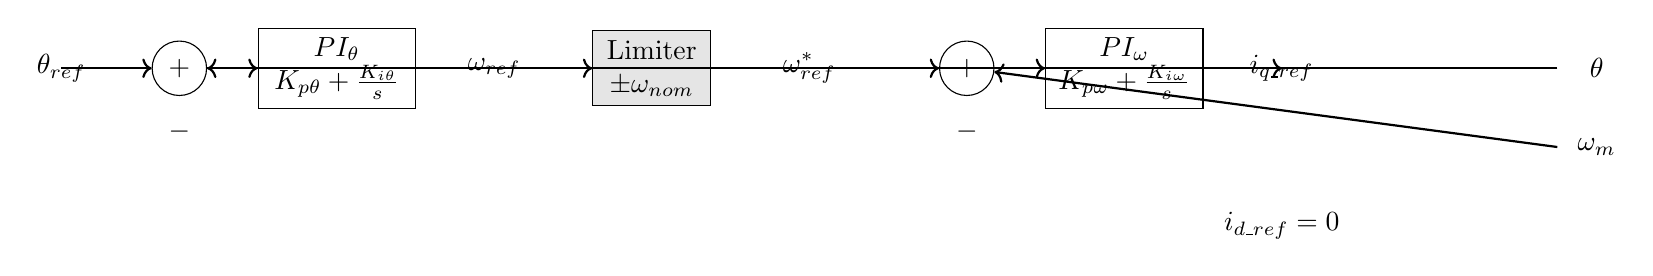
\begin{tikzpicture}[
    block/.style={rectangle, draw, minimum width=2cm, minimum height=1cm, align=center},
    limiter/.style={rectangle, draw, minimum width=1.5cm, minimum height=0.8cm, align=center, fill=gray!20},
    sum/.style={circle, draw, minimum size=0.5cm},
    arrow/.style={->, thick}
]

% Input
\node at (0,0) {$\theta_{ref}$};

% Position error
\node[sum] (sum1) at (1.5,0) {+};
\node at (1.5,-0.8) {$-$};

% Position PI Controller
\node[block] (PItheta) at (3.5,0) {$PI_\theta$ \\ $K_{p\theta} + \frac{K_{i\theta}}{s}$};

% Speed reference
\node at (5.5,0) {$\omega_{ref}$};

% Speed limiter
\node[limiter] (limiter) at (7.5,0) {Limiter \\ $\pm\omega_{nom}$};

% Limited speed reference
\node at (9.5,0) {$\omega_{ref}^*$};

% Speed error
\node[sum] (sum2) at (11.5,0) {+};
\node at (11.5,-0.8) {$-$};

% Speed PI Controller
\node[block] (PIomega) at (13.5,0) {$PI_\omega$ \\ $K_{p\omega} + \frac{K_{i\omega}}{s}$};

% Current reference
\node at (15.5,0) {$i_{q\_ref}$};

% d-axis reference
\node at (15.5,-2) {$i_{d\_ref} = 0$};

% Arrows
\draw[arrow] (0,0) -- (sum1);
\draw[arrow] (sum1) -- (PItheta);
\draw[arrow] (PItheta) -- (limiter);
\draw[arrow] (limiter) -- (sum2);
\draw[arrow] (sum2) -- (PIomega);
\draw[arrow] (PIomega) -- (15.5,0);

% Feedback from position
\draw[arrow] (19,0) -- (sum1);
\node at (19.5,0) {$\theta$};

% Feedback from speed
\draw[arrow] (19,-1) -- (sum2);
\node at (19.5,-1) {$\omega_m$};

\end{tikzpicture}
\caption{Üst Düzey Hiyerarşi - Konum ve Hız Kontrol Döngüleri}
\end{figure}

\subsection*{2. Elektrik İç Döngüler - d-q Akım Kontrolü ve Decoupling}

\begin{figure}[H]
\centering
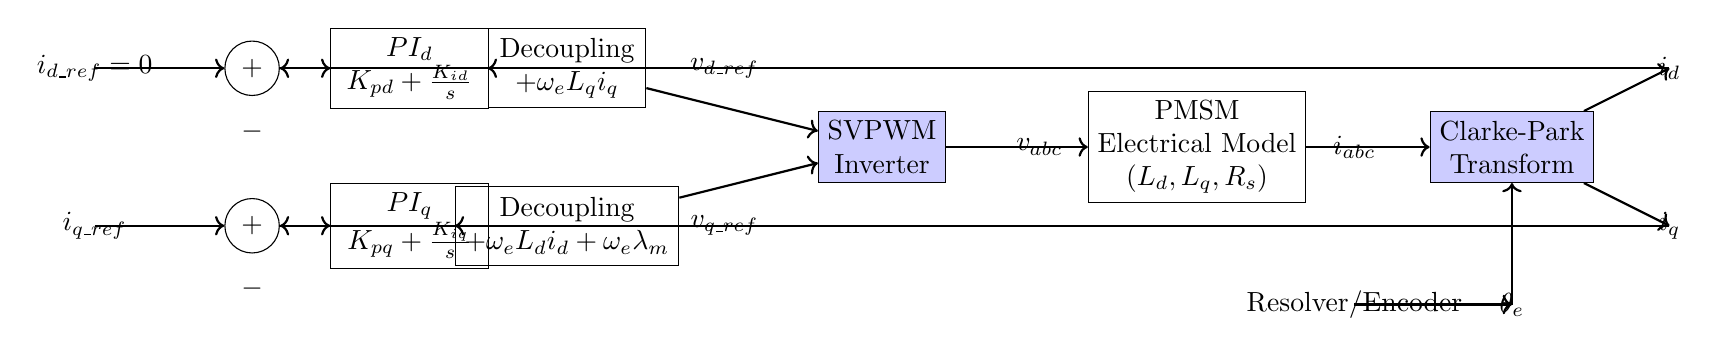
\begin{tikzpicture}[
    block/.style={rectangle, draw, minimum width=2cm, minimum height=1cm, align=center},
    sum/.style={circle, draw, minimum size=0.5cm},
    arrow/.style={->, thick},
    transform/.style={rectangle, draw, minimum width=1.5cm, minimum height=0.8cm, align=center, fill=blue!20}
]

% Current references
\node at (0,2) {$i_{d\_ref} = 0$};
\node at (0,0) {$i_{q\_ref}$};

% Current errors
\node[sum] (sum_d) at (2,2) {+};
\node at (2,1.2) {$-$};
\node[sum] (sum_q) at (2,0) {+};
\node at (2,-0.8) {$-$};

% PI Controllers
\node[block] (PI_d) at (4,2) {$PI_d$ \\ $K_{pd} + \frac{K_{id}}{s}$};
\node[block] (PI_q) at (4,0) {$PI_q$ \\ $K_{pq} + \frac{K_{iq}}{s}$};

% Decoupling terms
\node[block] (dec_d) at (6,2) {Decoupling \\ $+\omega_e L_q i_q$};
\node[block] (dec_q) at (6,0) {Decoupling \\ $+\omega_e L_d i_d + \omega_e \lambda_m$};

% Voltage references
\node at (8,2) {$v_{d\_ref}$};
\node at (8,0) {$v_{q\_ref}$};

% SVPWM/Inverter
\node[transform] (svpwm) at (10,1) {SVPWM \\ Inverter};

% Three-phase voltages
\node at (12,1) {$v_{abc}$};

% PMSM Electrical Model
\node[block] (pmsm) at (14,1) {PMSM \\ Electrical Model \\ $(L_d, L_q, R_s)$};

% Three-phase currents
\node at (16,1) {$i_{abc}$};

% Clarke-Park Transform
\node[transform] (clarke_park) at (18,1) {Clarke-Park \\ Transform};

% d-q currents
\node at (20,2) {$i_d$};
\node at (20,0) {$i_q$};

% Electrical angle
\node at (18,-1) {$\theta_e$};
\node at (16,-1) {Resolver/Encoder};

% Arrows
\draw[arrow] (0,2) -- (sum_d);
\draw[arrow] (0,0) -- (sum_q);
\draw[arrow] (sum_d) -- (PI_d);
\draw[arrow] (sum_q) -- (PI_q);
\draw[arrow] (PI_d) -- (dec_d);
\draw[arrow] (PI_q) -- (dec_q);
\draw[arrow] (dec_d) -- (svpwm);
\draw[arrow] (dec_q) -- (svpwm);
\draw[arrow] (svpwm) -- (pmsm);
\draw[arrow] (pmsm) -- (clarke_park);
\draw[arrow] (clarke_park) -- (20,2);
\draw[arrow] (clarke_park) -- (20,0);

% Feedback arrows
\draw[arrow] (20,2) -- (sum_d);
\draw[arrow] (20,0) -- (sum_q);

% Electrical angle feedback
\draw[arrow] (16,-1) -- (18,-1);
\draw[arrow] (18,-1) -- (clarke_park);

\end{tikzpicture}
\caption{Elektrik İç Döngüler - d-q Akım Kontrolü ve Decoupling}
\end{figure}

\subsection*{3. Mekanik Model ve Hız Geri Beslemesi}

\begin{figure}[H]
\centering
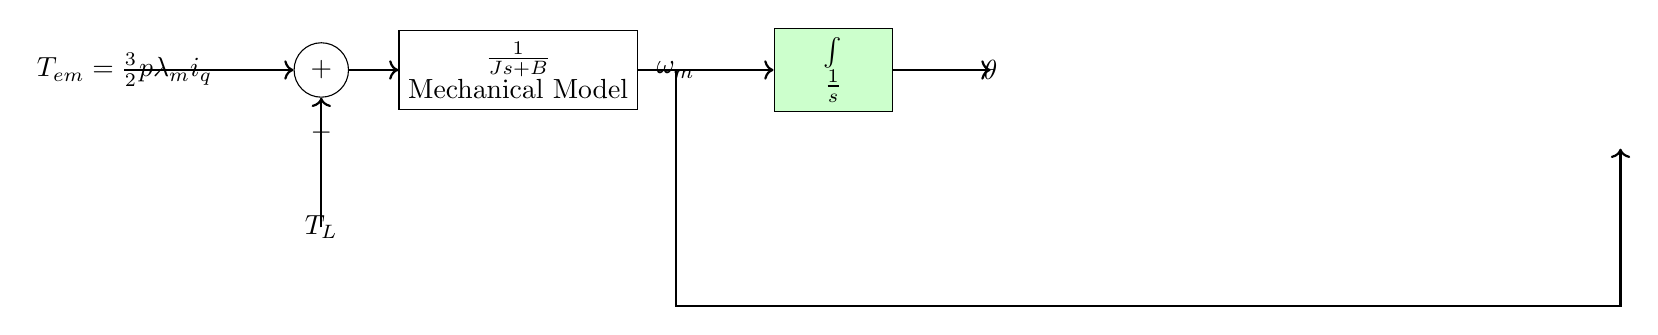
\begin{tikzpicture}[
    block/.style={rectangle, draw, minimum width=2cm, minimum height=1cm, align=center},
    sum/.style={circle, draw, minimum size=0.5cm},
    arrow/.style={->, thick},
    integrator/.style={rectangle, draw, minimum width=1.5cm, minimum height=0.8cm, align=center, fill=green!20}
]

% Electromagnetic torque
\node at (0,0) {$T_{em} = \frac{3}{2}p\lambda_m i_q$};

% Torque difference
\node[sum] (sum_torque) at (2.5,0) {+};
\node at (2.5,-0.8) {$-$};

% Load torque
\node at (2.5,-2) {$T_L$};

% Mechanical model
\node[block] (mech) at (5,0) {$\frac{1}{Js + B}$ \\ Mechanical Model};

% Mechanical speed
\node at (7,0) {$\omega_m$};

% Integrator
\node[integrator] (int) at (9,0) {$\int$ \\ $\frac{1}{s}$};

% Position
\node at (11,0) {$\theta$};

% Arrows
\draw[arrow] (0,0) -- (sum_torque);
\draw[arrow] (2.5,-2) -- (sum_torque);
\draw[arrow] (sum_torque) -- (mech);
\draw[arrow] (mech) -- (int);
\draw[arrow] (int) -- (11,0);

% Speed feedback
\draw[arrow] (7,0) -- (7,-3) -- (19,-3) -- (19,-1);

\end{tikzpicture}
\caption{Mekanik Model ve Hız Geri Beslemesi}
\end{figure}

\subsection*{4. Nominal Hız Koruması - Limiter Detayı}

\begin{figure}[H]
\centering
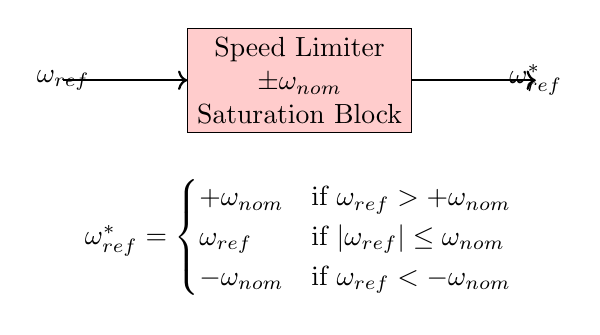
\begin{tikzpicture}[
    block/.style={rectangle, draw, minimum width=2cm, minimum height=1cm, align=center},
    limiter/.style={rectangle, draw, minimum width=2.5cm, minimum height=1.2cm, align=center, fill=red!20},
    arrow/.style={->, thick}
]

% Input speed reference
\node at (0,0) {$\omega_{ref}$};

% Limiter block
\node[limiter] (limiter) at (3,0) {Speed Limiter \\ $\pm\omega_{nom}$ \\ Saturation Block};

% Limited output
\node at (6,0) {$\omega_{ref}^*$};

% Arrows
\draw[arrow] (0,0) -- (limiter);
\draw[arrow] (limiter) -- (6,0);

% Limiter function
\node at (3,-2) {$\omega_{ref}^* = \begin{cases}
+\omega_{nom} & \text{if } \omega_{ref} > +\omega_{nom} \\
\omega_{ref} & \text{if } |\omega_{ref}| \leq \omega_{nom} \\
-\omega_{nom} & \text{if } \omega_{ref} < -\omega_{nom}
\end{cases}$};

\end{tikzpicture}
\caption{Nominal Hız Koruması - Limiter Fonksiyonu}
\end{figure}

\subsection*{5. Tam Sistem Blok Diyagramı - Entegre Yapı}

\begin{figure}[H]
\centering
\begin{tikzpicture}[
    block/.style={rectangle, draw, minimum width=2cm, minimum height=1cm, align=center},
    sum/.style={circle, draw, minimum size=0.5cm},
    arrow/.style={->, thick},
    transform/.style={rectangle, draw, minimum width=1.5cm, minimum height=0.8cm, align=center, fill=blue!20},
    limiter/.style={rectangle, draw, minimum width=1.5cm, minimum height=0.8cm, align=center, fill=red!20},
    integrator/.style={rectangle, draw, minimum width=1.5cm, minimum height=0.8cm, align=center, fill=green!20}
]

% Position reference
\node at (0,4) {$\theta_{ref}$};

% Position error
\node[sum] (sum_pos) at (1.5,4) {+};
\node at (1.5,3.2) {$-$};

% Position PI
\node[block] (PI_pos) at (3.5,4) {$PI_\theta$};

% Speed reference
\node at (5.5,4) {$\omega_{ref}$};

% Speed limiter
\node[limiter] (speed_lim) at (7.5,4) {Limiter};

% Limited speed
\node at (9.5,4) {$\omega_{ref}^*$};

% Speed error
\node[sum] (sum_speed) at (11.5,4) {+};
\node at (11.5,3.2) {$-$};

% Speed PI
\node[block] (PI_speed) at (13.5,4) {$PI_\omega$};

% Current reference
\node at (15.5,4) {$i_{q\_ref}$};

% d-axis reference
\node at (15.5,2) {$i_{d\_ref} = 0$};

% Current errors
\node[sum] (sum_id) at (17.5,2) {+};
\node at (17.5,1.2) {$-$};
\node[sum] (sum_iq) at (17.5,4) {+};
\node at (17.5,3.2) {$-$};

% Current PI controllers
\node[block] (PI_d) at (19.5,2) {$PI_d$};
\node[block] (PI_q) at (19.5,4) {$PI_q$};

% Decoupling
\node[block] (dec_d) at (21.5,2) {Decoupling};
\node[block] (dec_q) at (21.5,4) {Decoupling};

% Voltage references
\node at (23.5,2) {$v_{d\_ref}$};
\node at (23.5,4) {$v_{q\_ref}$};

% SVPWM
\node[transform] (svpwm) at (25.5,3) {SVPWM};

% PMSM
\node[block] (pmsm) at (27.5,3) {PMSM};

% Clarke-Park
\node[transform] (clarke_park) at (29.5,3) {Clarke-Park};

% d-q currents
\node at (31.5,2) {$i_d$};
\node at (31.5,4) {$i_q$};

% Torque
\node at (33.5,3) {$T_{em}$};

% Mechanical model
\node[block] (mech) at (35.5,3) {$\frac{1}{Js + B}$};

% Speed
\node at (37.5,3) {$\omega_m$};

% Integrator
\node[integrator] (int) at (39.5,3) {$\int$};

% Position
\node at (41.5,3) {$\theta$};

% Encoder
\node at (37.5,1) {Encoder};

% Electrical angle
\node at (39.5,1) {$\theta_e$};

% Arrows - Main path
\draw[arrow] (0,4) -- (sum_pos);
\draw[arrow] (sum_pos) -- (PI_pos);
\draw[arrow] (PI_pos) -- (speed_lim);
\draw[arrow] (speed_lim) -- (sum_speed);
\draw[arrow] (sum_speed) -- (PI_speed);
\draw[arrow] (PI_speed) -- (15.5,4);
\draw[arrow] (15.5,4) -- (sum_iq);
\draw[arrow] (15.5,2) -- (sum_id);
\draw[arrow] (sum_id) -- (PI_d);
\draw[arrow] (sum_iq) -- (PI_q);
\draw[arrow] (PI_d) -- (dec_d);
\draw[arrow] (PI_q) -- (dec_q);
\draw[arrow] (dec_d) -- (svpwm);
\draw[arrow] (dec_q) -- (svpwm);
\draw[arrow] (svpwm) -- (pmsm);
\draw[arrow] (pmsm) -- (clarke_park);
\draw[arrow] (clarke_park) -- (31.5,2);
\draw[arrow] (clarke_park) -- (31.5,4);
\draw[arrow] (31.5,4) -- (33.5,3);
\draw[arrow] (33.5,3) -- (mech);
\draw[arrow] (mech) -- (int);
\draw[arrow] (int) -- (41.5,3);

% Feedback arrows
\draw[arrow] (41.5,3) -- (sum_pos);
\draw[arrow] (37.5,3) -- (sum_speed);
\draw[arrow] (31.5,2) -- (sum_id);
\draw[arrow] (31.5,4) -- (sum_iq);

% Encoder feedback
\draw[arrow] (37.5,1) -- (39.5,1);
\draw[arrow] (39.5,1) -- (clarke_park);

\end{tikzpicture}
\caption{Tam SPMSM Konum Kontrol Sistemi Blok Diyagramı}
\end{figure}

\section*{Sistem Bileşenleri ve Açıklamaları}

\subsection*{Kontrol Döngüleri Hiyerarşisi}

\begin{enumerate}
    \item \textbf{Konum Döngüsü (Position Loop)}: $\theta_{ref} \rightarrow PI_\theta \rightarrow \omega_{ref}$
    \begin{itemize}
        \item Konum hatasını sıfıra indirir
        \item Hız referansı üretir
        \item $PI_\theta = K_{p\theta} + \frac{K_{i\theta}}{s}$
    \end{itemize}

    \item \textbf{Hız Döngüsü (Speed Loop)}: $\omega_{ref} \rightarrow \text{Limiter} \rightarrow PI_\omega \rightarrow i_{q\_ref}$
    \begin{itemize}
        \item Nominal hızı geçmemek için limiter sonrası çalışır
        \item $PI_\omega = K_{p\omega} + \frac{K_{i\omega}}{s}$
    \end{itemize}

    \item \textbf{Akım Döngüleri (Current Loops)}: $i_{d\_ref}, i_{q\_ref} \rightarrow PI_d, PI_q \rightarrow v_{d\_ref}, v_{q\_ref}$
    \begin{itemize}
        \item $i_{d\_ref} = 0$ (SPMSM'de MTPA = $I_d = 0$)
        \item $i_{q\_ref}$ tork üretir
        \item $PI_d = K_{pd} + \frac{K_{id}}{s}$, $PI_q = K_{pq} + \frac{K_{iq}}{s}$
    \end{itemize}
\end{enumerate}

\subsection*{Decoupling ve EMF Kompanzasyonu}

\begin{itemize}
    \item \textbf{d-ekseni Decoupling}: $+\omega_e L_q i_q$
    \item \textbf{q-ekseni Decoupling}: $+\omega_e L_d i_d + \omega_e \lambda_m$
    \item \textbf{EMF Kompanzasyonu}: $\omega_e \lambda_m$ terimi
\end{itemize}

\subsection*{Dönüşümler ve Modeller}

\begin{itemize}
    \item \textbf{Clarke-Park Dönüşümü}: Üç faz akım $\rightarrow$ d-q bileşenleri
    \item \textbf{SVPWM/Sine-PWM}: $(v_d, v_q) \rightarrow v_{\alpha\beta} \rightarrow v_{abc}$
    \item \textbf{PMSM Elektrik Modeli}: $(L_d, L_q, R_s)$ parametreleri
    \item \textbf{Mekanik Model}: $\frac{1}{Js + B}$ (Atalet ve sürtünme)
\end{itemize}

\subsection*{Güvenlik ve Kısıtlamalar}

\begin{itemize}
    \item \textbf{Hız Limiteri}: $\pm\omega_{nom}$ sınırında hız referansını keser
    \item \textbf{Akım Limiterleri}: Motor ve inverter güvenliği için
    \item \textbf{Voltaj Limiterleri}: DC bus voltajı sınırları
\end{itemize}

\section*{Sınavda Yazılacak Önemli Terimler}

\begin{center}
\begin{tabular}{|l|l|l|}
\hline
\textbf{Kutu İçeriği} & \textbf{Matematiksel Gösterim} & \textbf{Açıklama} \\
\hline
$PI_\theta$ & $K_{p\theta} + \frac{K_{i\theta}}{s}$ & Konum kontrolcüsü \\
$PI_\omega$ & $K_{p\omega} + \frac{K_{i\omega}}{s}$ & Hız kontrolcüsü \\
$PI_d$ & $K_{pd} + \frac{K_{id}}{s}$ & d-ekseni akım kontrolcüsü \\
$PI_q$ & $K_{pq} + \frac{K_{iq}}{s}$ & q-ekseni akım kontrolcüsü \\
Decoupling & $+\omega_e L_q i_q$ vb. & İleri besleme terimleri \\
Limiter & $\pm\omega_{nom}$ & Hız sınırlayıcı \\
PMSM mech & $\frac{1}{Js + B}$ & Atalet bloğu \\
\hline
\end{tabular}
\end{center}

\end{document}
